%%%%%%%%%%%%%%%%%%%%%%%%%%%%%%%%%%%%%%%%%%%%%%%%%%%%%%%%%%%%%%%%%%%%%%%%%%%%%%%%
%									OPTIMAL MODEL							   %
%%%%%%%%%%%%%%%%%%%%%%%%%%%%%%%%%%%%%%%%%%%%%%%%%%%%%%%%%%%%%%%%%%%%%%%%%%%%%%%%
In this section, we address the evaluator's interpretation problem in the ideal situation when the conditional distribution \(\MLmodel^\star = \prob{\Z \given \XXX}\) is known -- \ie{} when the model is perfect -- where \(\XXX\) is the random variable denoting the observed trace and \(\Z\) is the random variable denoting the sensitive intermediate computation carrying information about the secret key.
We will show how the study of the derivatives of such a model with respect to each coordinate of an input trace can highlight information about our \glspl{poi}. 
To this end, we need two assumptions.

% First hypothesis
The first one is \autoref{assum:sparsity} and has already been stated in \autoref{sec:characterization}.
Informally, it tells that the leaking information is non-uniformly distributed over the trace, \ie{},  only a few coordinates contain clues about the attacked sensitive variable.
\autoref{assum:sparsity} has been already made \eg{} by Cagli \etal{}~\cite{cagli_enhancing_2016}.
Depending on the counter-measures implemented into the attacked device, the nature of \(\infoCoord\) may be precised. 
Without any counter-measure, and supposing that the target sensitive variable only leaks once, \autoref{assum:sparsity} states that \(\infoCoord\) is only a set of contiguous and constant coordinates, regardless the input traces.

In the case where the target implementation is protected by secret-sharing, \(\infoCoord\) will be split into several contiguous and fixed sets whose number is equal to the number of shares in the masking scheme (or at least equal to the number of shares if we relax the hypothesis of one leakage per share).
For example if \(\Z_1, \Z_2\), leaking respectively at the times samples \(t_1\) and \(t_2\), represent a \(2\)-sharing of \(\Z\), then \(\Z_1\) and \(\XXX[t]\) with \(t \neq t_1\) are independent (resp. \(\Z_2\) and \(\XXX[t]\) with \(t \neq t_2\) are independent). 
The conditional probability \(\prob{\Z = \sensValue \given \XXX = \xxx}\) satisfies for every \(\sensValue_2 \in \sensVarSet\):
\begin{multline}
	\MLmodel^\star(\xxx)[\sensValue] = \prob{\Z = \sensValue \given \XXX = \xxx} = \\
	\sum_{\substack{\sensValue_1, \sensValue_2 \in \sensVarSet \\ \fonction{\mathsf{Dec}}{\sensValue_1, \sensValue_2} = \sensValue}} \prob{\Z_1 = \sensValue_1 \given \XXX[t_1] = \xxx[t_1]} \prob{\Z_2 = \sensValue_2 \given \XXX[t_2] = \xxx[t_2]} \enspace .
\end{multline}
Adding de-synchronization should force \(\infoCoord\) to be non-constant between each 
trace.

% Second hypothesis
The second assumption is the following.
\begin{assum}[Regularity]\label{assum:deriv}
	The conditional probability distribution \(\MLmodel^\star\) is differentiable over \(\leakSpace\) and thereby continuous.
\end{assum}
Likewise, \autoref{assum:deriv} is realistic because it is a direct corollary of a Gaussian leakage assumption for the traces -- see \autoref{sec:profiled_attacks}.
It implies that \(\xxx \mapsto \prob{\XXX = \xxx \given \Z = \sensValue}\) is differentiable and:
\begin{eqnarray}\label{eq:GTA}
	\nabla_{\xxx} \prob{\XXX = \xxx \given \Z = \sensValue} & = & 
	\vectObs{\Sigma}_{\sensValue}^{-1} (\xxx - \vectObs{M}_{\sensValue}) \prob{\XXX = \xxx \given 
	\Z = \sensValue} \enspace ,
\end{eqnarray}
where \(\vectObs{M}_{\sensValue}\) and \(\vectObs{\Sigma}_{\sensValue}^{-1}\) respectively denote the mean vector and the covariance matrix of the normal probability distribution related to the target sensitive value hypothesis \(\sensValue\).
Then, from Bayes' theorem -- see \autoref{sec:probas}, \autoref{eq:GTA} and the basic rules for derivatives computation, it gives an analytic expression of \(\nabla_{\xxx}\MLmodel^\star(\xxx)\), thereby proving that \(\MLmodel^\star\) is differentiable with respect to the input trace.


\begin{figure}
	\centering
	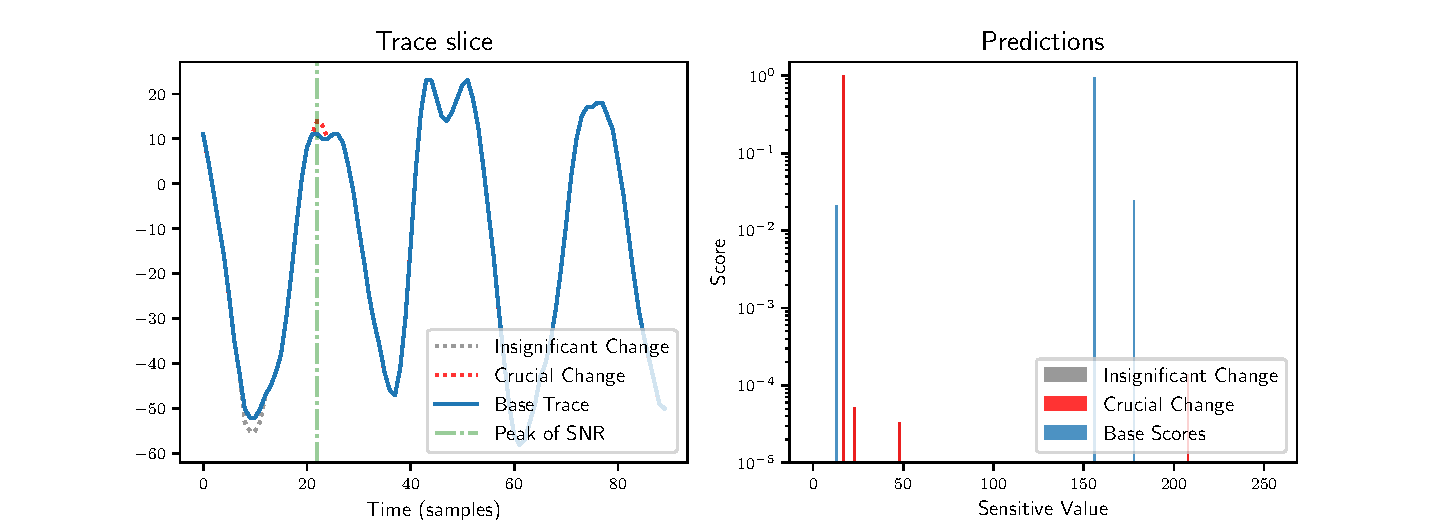
\includegraphics[width=\textwidth]{figures/Illustrations/optimal_model_illustration_review_backup.pdf}
	\caption{Illustration of the Sensitivity Analysis principle. 
	Left: a piece of trace. \(t \in \infoCoord\) is depicted by the green line, and slight variations dotted in red and gray.
	Right: predictions of the optimal model.}
	\label{fig:illustration_cosade}
\end{figure}
Once Assumptions~\ref{assum:sparsity} and~\ref{assum:deriv} are stated, we may want to observe their impact on the properties verified by the optimal model derivatives.
For such a purpose we start by considering an example on a trace \(\xxx\).
\autoref{fig:illustration_cosade} (left) illustrates such a trace in blue, and the green line depicts a \gls{poi}, namely a peak of \gls{snr} -- in other words the set of \glspl{poi} \(\infoCoord\) is reduced to a single time index. 
The \gls{pmf} returned by the optimal model \(\MLmodel^\star(\xxx)\) is given at the right of the same figure: it is here represented by the blue histogram over the 256 possible values of a byte.
We may fairly suppose that a slight variation on one coordinate not belonging to \(\infoCoord\) -- dotted in gray in \autoref{fig:illustration_cosade} (left) -- should not radically change the output of the optimal model. 
The resulting \gls{pmf}, depicted by the gray histogram on \autoref{fig:illustration_cosade} (right) remains the same, as it is perfectly superposed to the blue histogram.
However, applying a slight variation on the coordinate from \(\infoCoord\) -- dotted in red in \autoref{fig:illustration_cosade} (left) -- may radically change the output distribution depicted by the red histogram in \autoref{fig:illustration_cosade} (right).


This example illustrates the more general idea that small variations applied to the trace at a coordinate \(t \in \infoCoord\) should radically change the output prediction whereas small variations at \(t \notin \infoCoord\) should have no impact.
As a consequence, if \(\MLmodel^\star\) is differentiable with respect to the input trace (according to \autoref{assum:deriv}), there should exist \(\sensValue \in \sensVarSet\) such that:
\begin{equation}
	\partDeriv{\xxx[t]} \MLmodel^\star(\xxx)[\sensValue]
	\begin{cases} 
		\neq 0 &\mbox{\gls{iff} } t \in \infoCoord \\
		\approx 0 & \mbox{\gls{iff} } t \notin \infoCoord
	\end{cases}.
\end{equation}
The latter observation can be stated in terms of the \gls{jacob} of the estimator, denoted as \(J_{\MLmodel^\star}(\xxx)\).
Its coefficients should be zero almost everywhere, except in columns \(t \in \infoCoord\):

\begin{equation}
	J_{\MLmodel^\star}(\xxx) = 
	\left(
	\begin{matrix}
		\textbf{0} & \ldots & \textbf{0} & \textbf{Y}_t & \textbf{0} & \ldots & \textbf{0}
	\end{matrix}
	\right) \enspace ,
	\label{eq:jacobian}
\end{equation}
where \(\textbf{Y}_t = \left( \partDeriv{\xxx[t]} \MLmodel^\star(\xxx)[\sensValue_1],
\partDeriv{\xxx[t]} \MLmodel^\star(\xxx)[\sensValue_2], \ldots, \partDeriv{\xxx[t]} \MLmodel^\star(\xxx)\left[\sensValue_{\card{\sensVarSet}}\right] \right)^\intercal\) and 
\(\textbf{0}\) denotes the zero column vector.


The properties verified by the \gls{jacob} matrix in \autoref{eq:jacobian} form the cornerstone of this chapter, as it implies that we can guess from this matrix whether a coordinate from an input trace belongs to \(\infoCoord\) or not, \ie{}, whether a coordinate has been recognized as a \gls{poi} when designing the optimal model \(\MLmodel^\star\).
Moreover, except \autoref{assum:sparsity}, no more assumption on the nature of the leakage model is required.